% \documentclass[12pt, twoside]{article}
\usepackage[letterpaper, margin=1in, headsep=0.2in]{geometry}
\setlength{\headheight}{0.6in}
%\usepackage[english]{babel}
\usepackage[utf8]{inputenc}
\usepackage{microtype}
\usepackage{amsmath}
\usepackage{amssymb}
%\usepackage{amsfonts}
\usepackage[nomessages]{fp} %\FPeval{\var-name}{2*sin(pi/6)}
\usepackage{siunitx} %units in math. eg 20\milli\meter
\usepackage{yhmath} % for arcs, overparenth command
\usepackage{tikz} %graphics
\usetikzlibrary{quotes, angles, arrows, arrows.meta}
\usepackage{graphicx} %consider setting \graphicspath{{images/}}
\usepackage{parskip} %no paragraph indent
\usepackage{enumitem}
\usepackage{multicol}
\usepackage{venndiagram}

\usepackage{fancyhdr}
\pagestyle{fancy}
\fancyhf{}
\renewcommand{\headrulewidth}{0pt} % disable the underline of the header
\raggedbottom
\hfuzz=2mm %suppresses overfull box warnings

\usepackage{hyperref}

\fancyhead[LE]{\thepage}
\fancyhead[RO]{\thepage \\ Name: \hspace{4cm} \,\\}
\fancyhead[LO]{BECA / Dr. Huson / Geometry\\*  Unit 9: Dilation \\* 21 March 2023}

\begin{document}

\subsubsection*{9.5 Pop Quiz: Unit conversions, area \hfill CCSS}
\begin{enumerate}[itemsep=3.5cm]
\begin{multicols}{2}
\item How many pounds is 48 ounces?
\item How many feet is 144 inches?
\item How many quarts of milk could be poured from a five gallon canister?
\item Convert 5 miles to feet.
\item What is the volume of a cube that is 18 inches on a side in terms of cubic feet?
\item If a gallon of paint would cover 80 square feet, how many gallons would be required to paint a wall twenty feet long by eight feet high?
\item Find the area of a triangle with a base of 4 inches and height of 6 inches. \vspace{2cm}
\item What is the area of a circle with a 7 centimeter raduis, to the \emph{nearest tenth of a square centimeter}.
\item 
\end{multicols} 

\newpage
\item Find the area of the quadrilateral shown.
  \begin{center}
    \begin{tikzpicture}[scale=0.8]
      \draw [help lines] (-10,-10) grid (10,10);
      \draw [thick, <->] (-10.4,0) -- (10.4,0) node [right] {$x$};
      \draw [thick, <->] (0,-10.4)--(0,10.4) node [above] {$y$};
      \draw [thick]
        (-4,1) node[below left] {$A$}--
        (-2,-3) node[below left] {$B$}--
        (8,3) node[below] {$C$}--
        (6,7) node[above] {$D$}--
        cycle;
    \end{tikzpicture}
  \end{center}
Is $ABCD$ a rectangle? Calculate the slopes of the four sides.

\end{enumerate}
\end{document}
